\documentclass[aspectratio=169,10pt]{beamer}\usetheme{default}\usecolortheme{seahorse}\setbeamertemplate{navigation symbols}{}\setbeamertemplate{footline}[frame number]
\usepackage[T1]{fontenc}\usepackage[utf8]{inputenc}\usepackage{helvet}\usepackage{booktabs}
\title{Parking around rue de Terrebonne}\subtitle{Supply, measured demand, and the survey\textquoteright{}s answers in context}\author{Terrebonne-open-sources (a resident of Côte-des-Neiges--Notre-Dame-de-Grâce)}\date{2026-11-08}
\begin{document}
\begin{frame}\titlepage\end{frame}
\begin{frame}{The question}\begin{itemize}
\item The survey counts respondents: who keeps a vehicle, who has an off-street place, where the car was last night, who met the winter-hardship definition.
\item The measurements that exist are of another kind: EXP\textquoteright{}s 2022 inventory and occupancy (two days), the cars at the curbs on a 2015 night and a daytime orthophoto, off-street parking building by building, the roll\textquoteright{}s dwellings, five winters of snow-removal nights.
\item What do they say about the population the respondents come from, which survey answers can be checked, and what remains unmeasured?
\end{itemize}\end{frame}
\begin{frame}{EXP 2022: occupancy by sector and period}\centering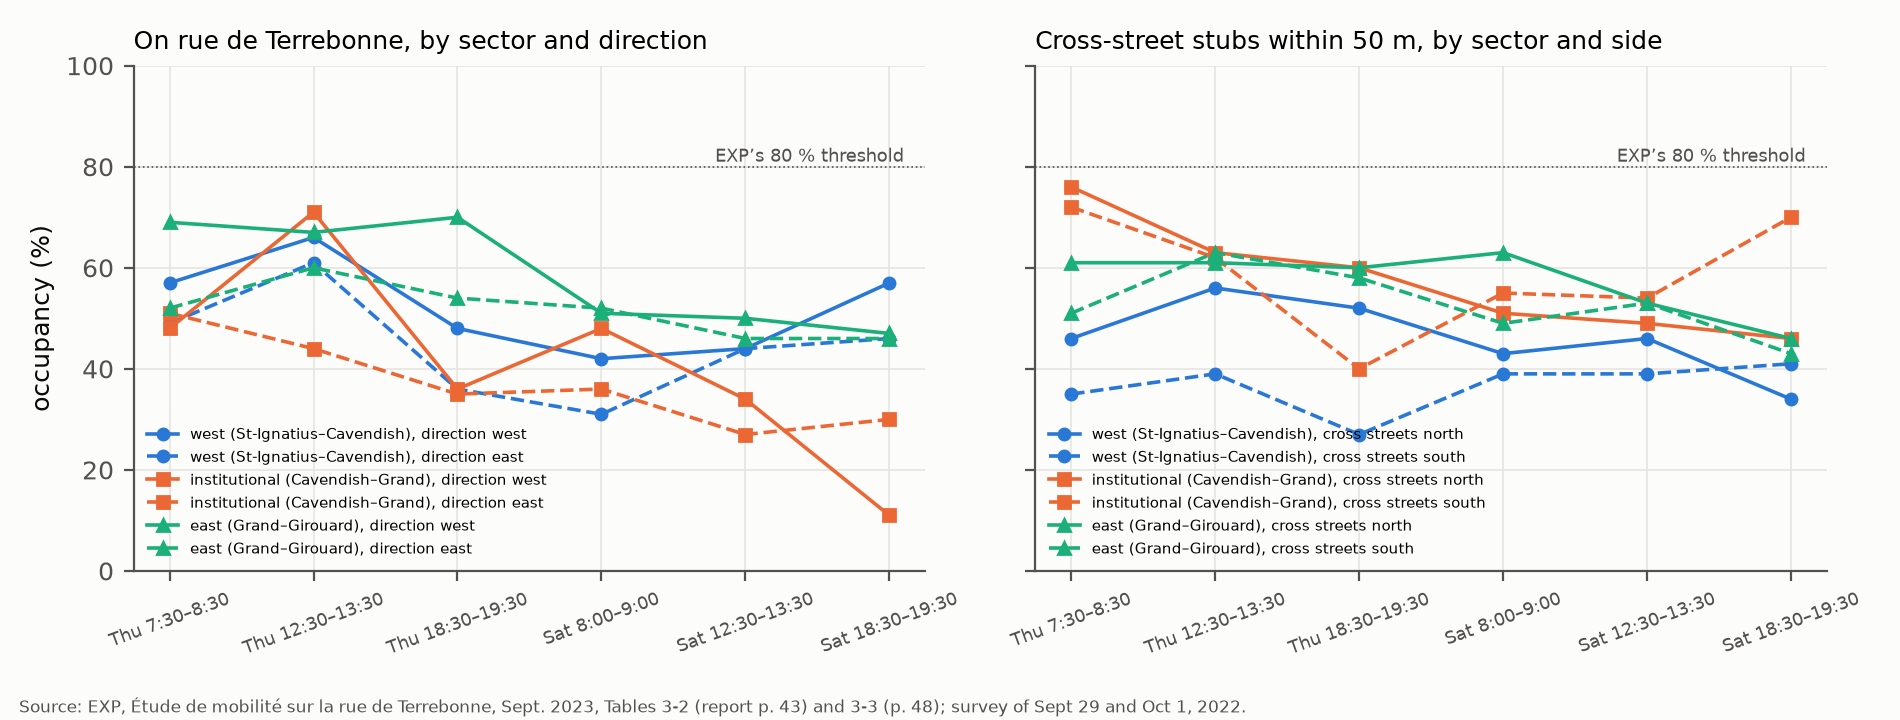
\includegraphics[width=0.95\textwidth]{figures/exp_occupancy_en.png}\\{\scriptsize Thursday Sept 29 and Saturday Oct 1, 2022; Tables 3-2 (p.~43) and 3-3 (p.~48). No cell above 71\,\% on Terrebonne; every sector below EXP\textquoteright{}s 80\,\% threshold at every period.}\end{frame}
\begin{frame}{EXP 2022: occupied and vacant places}\centering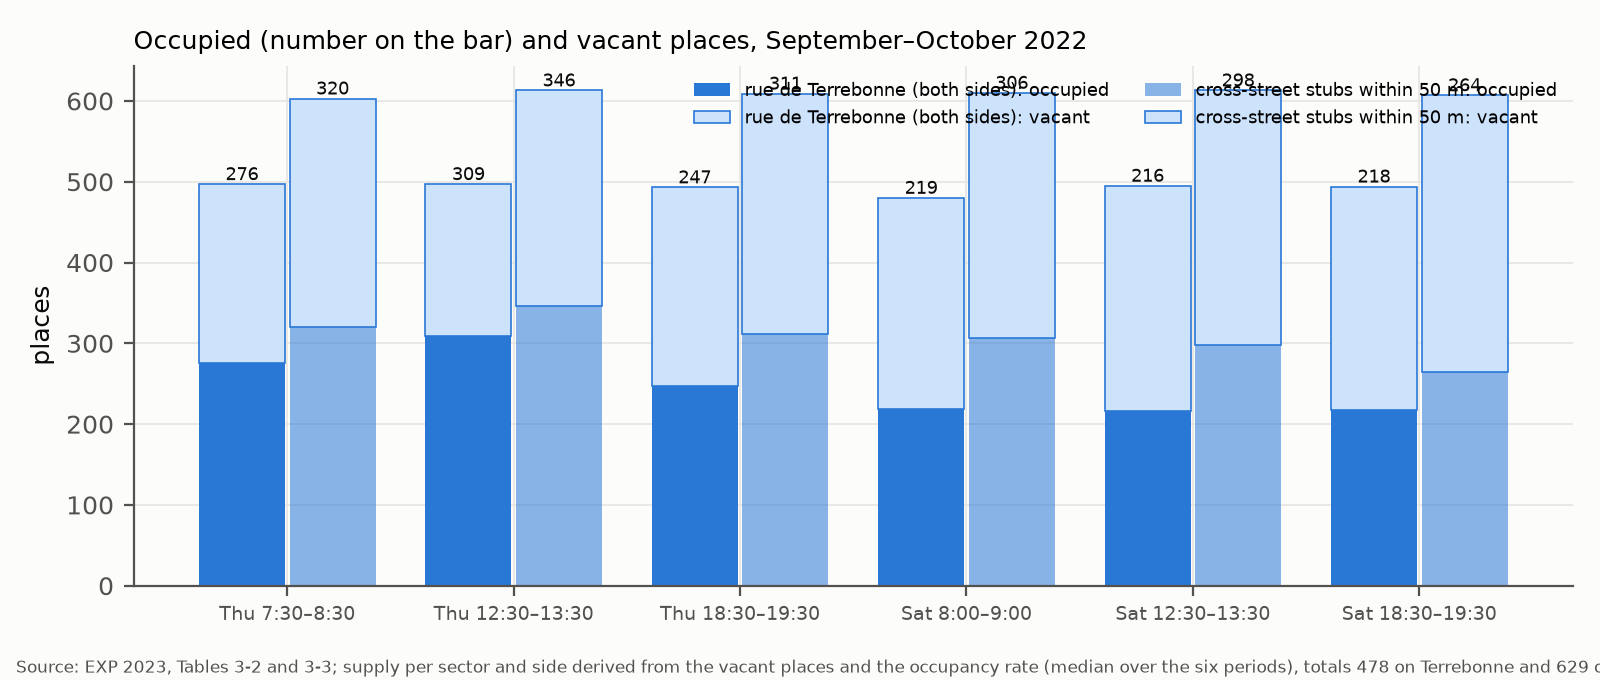
\includegraphics[width=0.85\textwidth]{figures/exp_occupied_vacant_en.png}\\{\scriptsize Thursday 18:30--19:30: 247 cars on Terrebonne (50\,\%), 246 places vacant there and 298 on the stubs. Supply per sector derived from the vacant places and the rate; stated totals 478 and 629 (p.~40).}\end{frame}
\begin{frame}{The cars at the curbs before the lane}\centering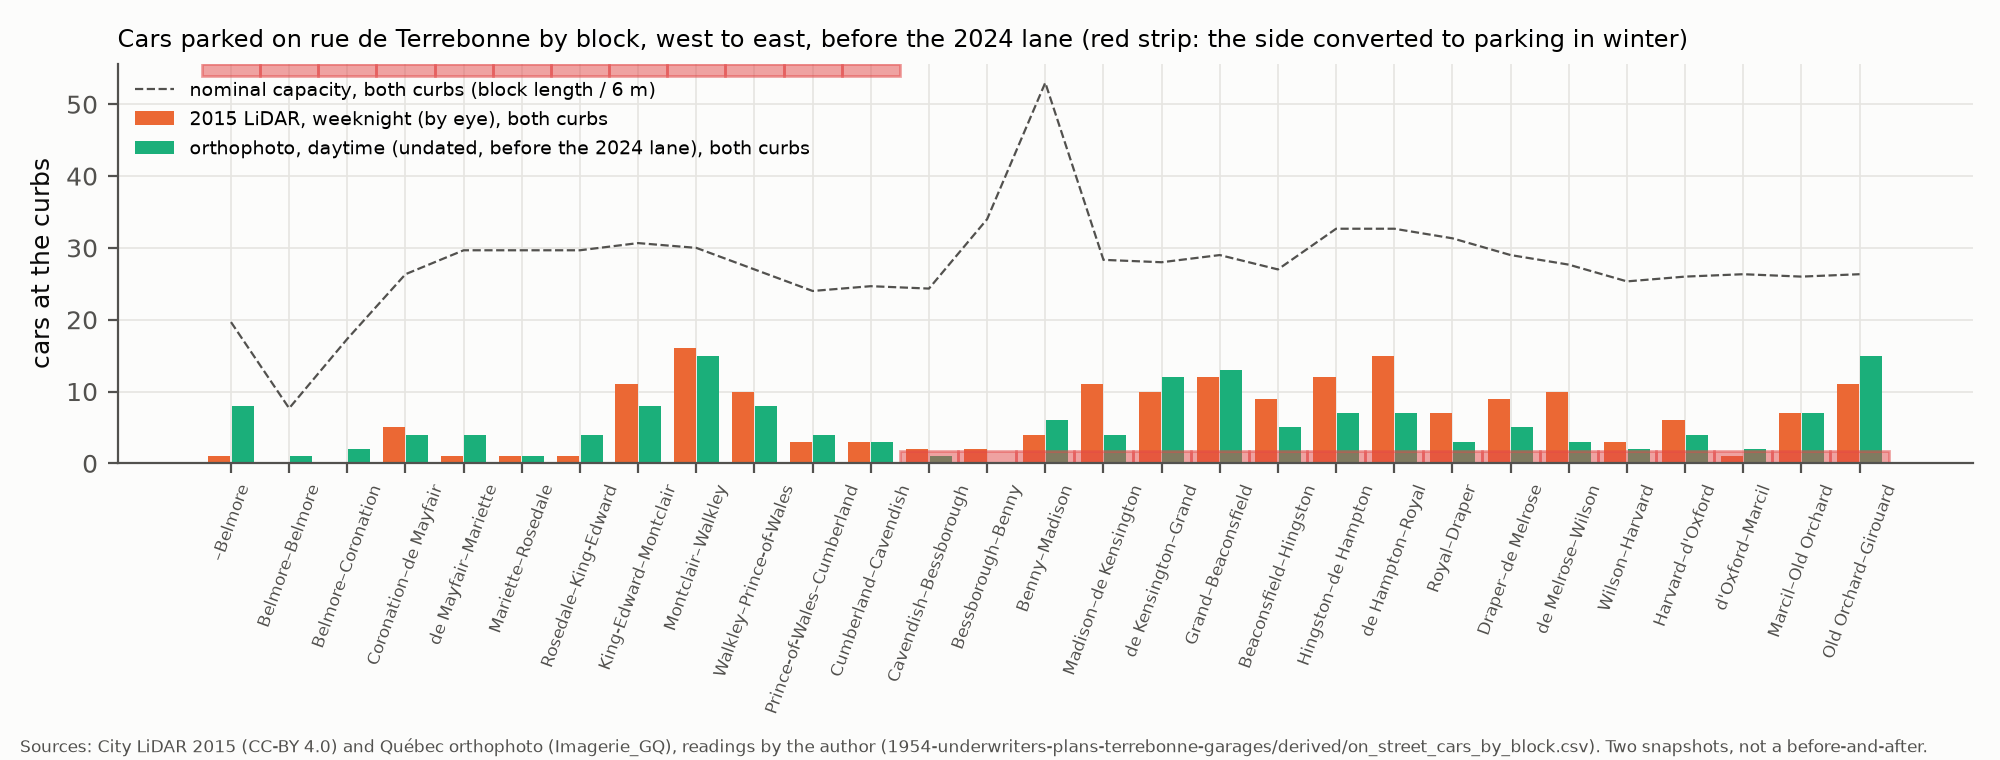
\includegraphics[width=\textwidth]{figures/curb_cars_by_block_en.png}\end{frame}
\begin{frame}{By sector: night 2015, EXP evening 2022, and today\textquoteright{}s one side}\centering\small\begin{tabular}{@{}lrrrrrr@{}}\toprule sector & blocks & EXP supply & EXP occupied, Thu 18:30 & LiDAR night 2015 & night / supply & orthophoto, day\\ \midrule
residential west & 12 & 189 & 79 & 52 & 28\,\% & 62 \\
institutional & 5 & 83 & 30 & 29 & 35\,\% & 23 \\
residential east & 12 & 223 & 138 & 102 & 46\,\% & 73 \\
\bottomrule\end{tabular}\\[6pt]\footnotesize Both measurements of demand before the lane (183 and 247 cars on Terrebonne) are of the order of the one parking band that remains today (about 239 places); below it in the west, near it in the east, with 298 places vacant on the stubs at the same hour in 2022. Nothing has been measured since the lane was built.\end{frame}
\begin{frame}{Off-street parking: a ground truth for one survey question}\centering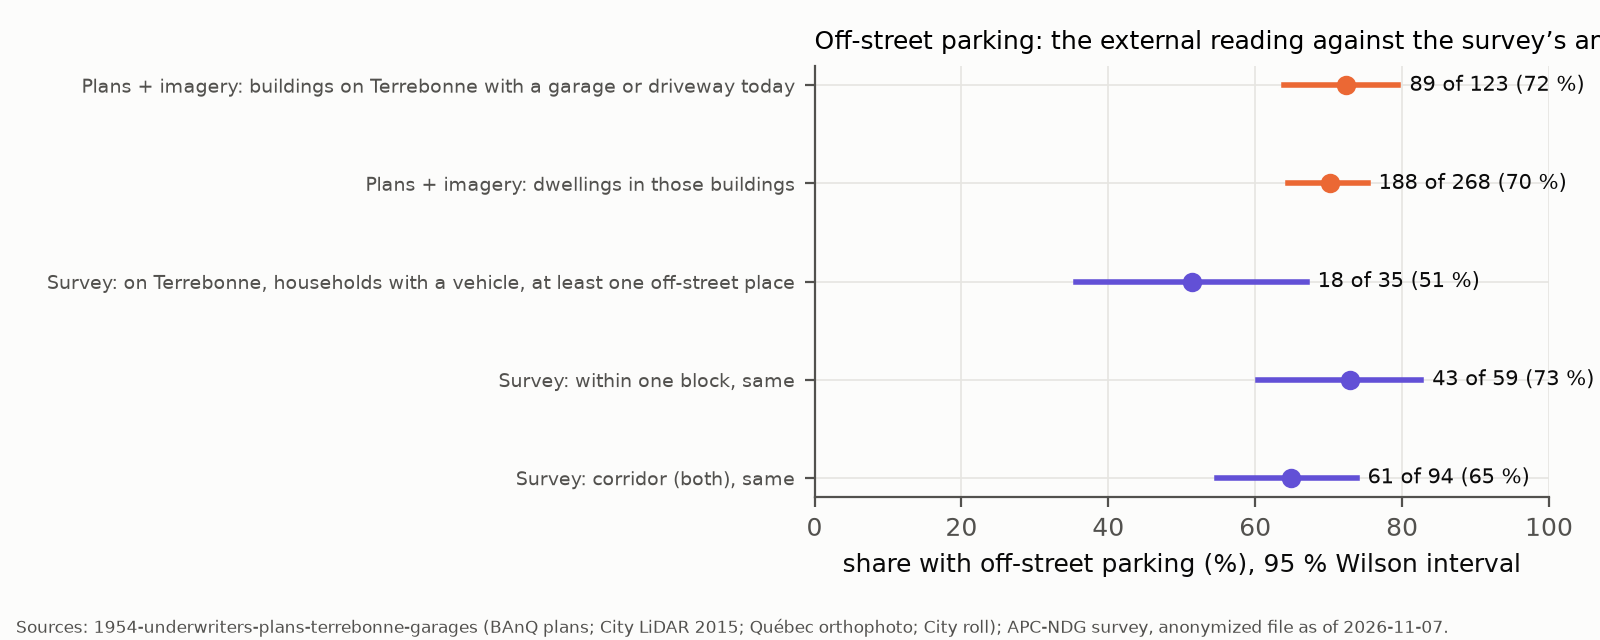
\includegraphics[width=0.9\textwidth]{figures/offstreet_share_en.png}\\{\scriptsize Seven in ten dwellings on Terrebonne have a garage or driveway. Respondents on the street report one in 18 of 35 households with a vehicle: at the low edge of the interval, as a survey about parking would be expected to show. Within a block, survey and reading agree.}\end{frame}
\begin{frame}{The survey\textquoteright{}s demand floor}\centering\scriptsize\resizebox{\textwidth}{!}{\begin{tabular}{@{}lrrrrrrrr@{}}\toprule group & respondents & with a vehicle & off-street place & own off-street last night & on Terrebonne & cross street within a block & street parkers & hardship strict / loose\\ \midrule
on Terrebonne & 37 & 35 & 18 of 35 & 15 & 9 & 9 & 22 & 17 / 19 \\
within one block & 72 & 59 & 43 of 59 & 25 & 6 & 32 & 38 & 18 / 28 \\
corridor (both) & 109 & 94 & 61 of 94 & 40 & 15 & 41 & 60 & 35 / 47 \\
all respondents & 206 & 157 & 106 of 156 & 75 & 16 & 56 & 82 & 43 / 64 \\
\bottomrule\end{tabular}}\\[6pt]\footnotesize Floors, in the filing\textquoteright{}s sense: at least this many answered this way. The roll holds 573 dwellings on Terrebonne and 5,029 within the Somerled--Monkland band; the survey reached 6\,\% and 1\,\% of them.\end{frame}
\begin{frame}{Where the car was parked last night}\centering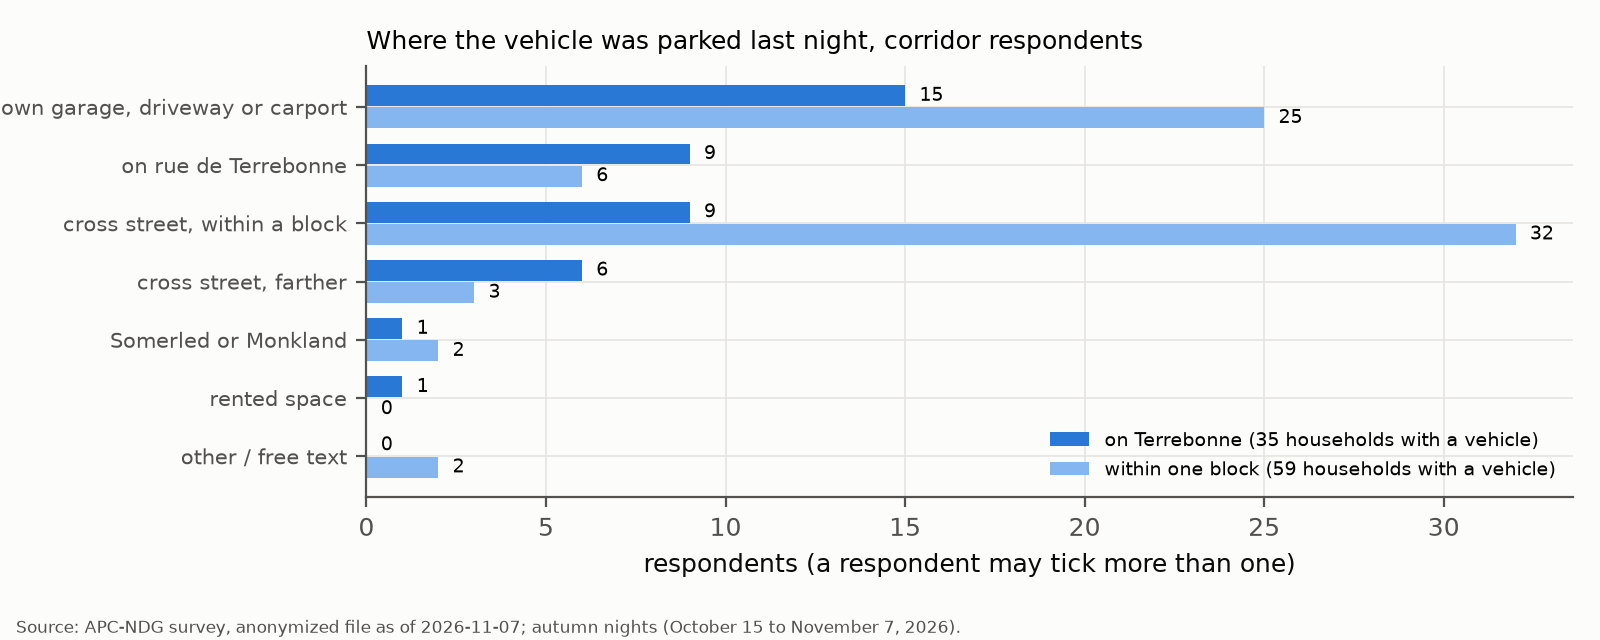
\includegraphics[width=0.85\textwidth]{figures/survey_parked_last_night_en.png}\end{frame}
\begin{frame}{The winters the hardship questions describe}\centering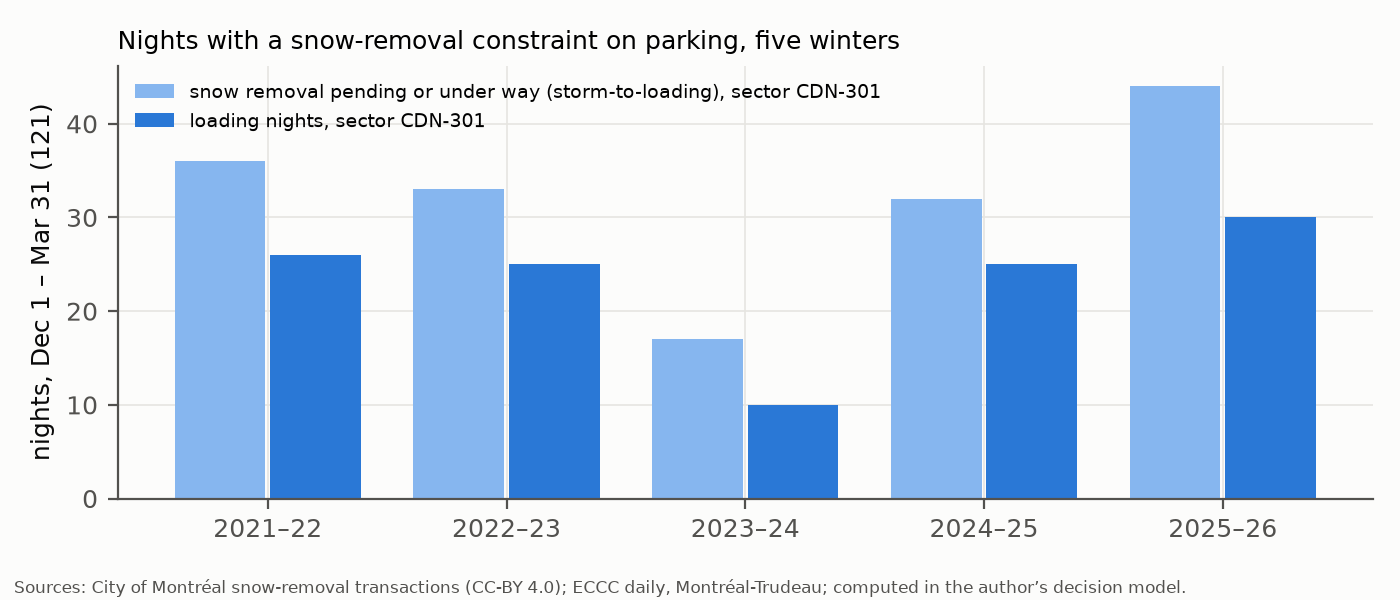
\includegraphics[width=0.75\textwidth]{figures/winter_constraint_nights_en.png}\\{\scriptsize Snow removal pending or under way on about 32 of 121 nights a winter in the sector, 23 with loading; stretches of three weeks or more without it every winter. The record gives how often the condition existed, not how often a respondent met it.}\end{frame}
\begin{frame}{What is settled, what is not}\begin{itemize}
\item Settled: before the lane, Terrebonne\textquoteright{}s parking was one-third to one-half full at the hours measured, fuller in the east; seven in ten dwellings have off-street parking; the one band that remains is of the order of the demand measured then.
\item The survey\textquoteright{}s parking counts sit inside those measurements and are floors, not rates; on the street itself the sample tilts toward households that park on the street.
\item Not settled: present occupancy with the lane in place (nothing counted since 2022); the hardship counts have no external check.
\item EXP\textquoteright{}s mandate of October 6, 2026 (due November 27) analyses supply, not occupancy. A night count on the remaining band and the cross streets would close the gap.
\item Code, tables, figures: \url{https://github.com/OpenMobilityData/Terrebonne-open-sources/tree/main/2026-parking-supply-demand-survey-context}
\end{itemize}\end{frame}
\end{document}
